\chapter{Subjective validation of auralisation method}\label{chapter:test}
% TODO From paper. Rewrite

\section{Introduction}
In the previous chapter an overview was given of the auralisation tool. A
propagation model for aircraft sound was developed but still missing is an
emission model. An algorithm was presented for extracting select features from
recordings with the underlying idea of using those features for the development
of an empirical emission model.

This chapter describes a listening test that was conducted. The purpose of the
listening test was to check the plausiblity or perceptual validity of the
auralisations and a comparison was therefore made between recordings and
auralisations.

The hypothesis is that \emph{recordings and auralisations of aircraft of the same
type and under similar conditions are samples of the same group}.
Audible differences are likely to occur and are also acceptable, because even
among recordings of the same aircraft type there are audible differences.

% TODO maybe drop this part?
How sounds are perceived can depend on many factors. Factors can be properties
of the sound, but also of the listener or the environment. Psychoacoustic
measures describe how a sound is perceived by most listeners and can therefore
be used to characterise a sound. Many measures exist, but not all measures are
appliceable to all sounds and care should therefore be taken when choosing
measures. Examples of common measures are loudness, roughness and sharpness.

Due to time-constraints psychoacoustic measures were not measured. Instead, an
overall similarity between stimuli was determined. Recordings were compared not
only with auralisations, but also with other recordings, and similarly,
auralisations with other auralisations. Each of these comparisons can be
considered a group. If the hypothesis is valid, then the distribution of the
group with comparisons between recordings and auralisations, should be the same
as the other two distributions.

% The purpose of the
% test was to determine whether the auralisation tool produces auralisations that
% sound similar to recordings, where the auralisations use for the emission
% synthesis features that were extracted from the recordings. Because the
% available data sets permits simulating and comparing different aircraft types,
% the purpose was also to test whether participants can distinguish between
% aircraft types.
%
% The purpose was not to determine similarity with respect to a certain aspect,
% like for example annoyance, but instead the overall similarity as the goal was to create a tool capable of

% TODO several methods

\section{Method} % This section has been rewritten...slightly.

The goal of the listening test was to determine whether the auralisations sound
similar to the recordings they were based on. Participants were presented with
pairs of stimuli and asked to rate how similar they sounded.

% TODO {explain why this method is chosen? Explain other available methods?}
% One can think of multiple methods to
% determine the similarity. The MUSHRA (MUltiple Stimuli with Hidden Reference and
% Anchor) test is methodology used for evaluating audio quality \cite{}, and has also been used for determining the plausibility of synthesised vehicle pass-by sounds when compared to recordings \cite{Southern2016}.

Eight different sounds were considered and they were each 12 seconds long. The
sounds include the approach of an aircraft, its flyover and its distancing.
Because the character of the sounds varies considerably over time, they were
each split into parts of four seconds, corresponding to the approach, fly-over
and distancing. The listening test was also divided in these three parts. First,
participants were presented to all approach stimuli, then all fly-over stimuli
and finally all distancing stimuli. In each test part all stimuli combinations
were considered. Therefore, each part consisted of 28 pairs of stimuli of four
seconds.

Of the eight sounds four were recordings, and four were auralisations. Each
auralisation was based on one of the recordings. Two aircraft types were
considered, an A320 and a RJ1H, as well as two events per aircraft type.
% The recordings were made close to the airport.
% TODO this sentence can be dropped if we have a Measurements section
% with the aircraft passing by at approximately 90 meters.
Fade in and fade out was applied to the stimuli. The signals were mono and
presented with headphones. Head-related transfer functions were not included.

Similarity is relative, and therefore an anchor is typically used. For each
part, participants were first given the set of stimuli, in order to become
familiar with the type of sounds and the spread in the sounds of that part, and
then continued with rating the pairs. The rating was done on an eleven point
Likert scale. The left side of the scale said ``not so much'' and the right side
``very much''. The scale was not numbered. The order of the stimuli was
randomised for each test and each part.

Figures \ref{fig:listening:results:recording-A320} and
\ref{fig:listening:results:simulation-A320} show spectrograms of some of the stimuli
that were used. The blade passing frequency and harmonics are not as prominent
in the auralisation as they are in the recording.

% \newpage
% \afterpage{
\begin{figure}[H]
  \centering
  \includegraphics[]{../figures/generated/listening/recording-A320}
  \caption{Spectrograms of the approach, fly-over and distancing parts of a recording of an A320.}
  \label{fig:listening:results:recording-A320}
% \end{figure}
%
% \begin{figure}
  \centering
  \includegraphics[]{../figures/generated/listening/turbulence-A320}
  \caption{Spectrograms of the approach, ``center`` and distancing parts of an auralisation of an A320.}
  \label{fig:listening:results:simulation-A320}
\end{figure}
% }
% \clearpage

\newpage
\section{Results}
The results of the participants were scaled linearly from 0 to 1 with 0
corresponding to ``not so much'' and 1 corresponding to ``very much''.
% Not all of the participants used the entire scale, and therefore they were rescaled per
% participant and per test part to use the full scale.
There were 17 participants, all graduate students, and of which the majority
studied acoustics. The results that are shown are obtained after joining the
data of all participants. % and all three test parts.
% Update raw results??
The listening test data can be found at \cite{Rietdijk2017a} and the
raw results along with a brief analysis at \cite{Rietdijk2017b}.

Table \ref{table:listening:results:analysis-parts} shows the mean $\mu$,
standard deviation $\sigma$ and amount of samples $n$ per group.
Averaging was done over participants. Table \ref{table:listening:results:analysis} is similar,
but with this table averaging was done not over only participants but also over the three test parts.

Figure \ref{fig:listening:ratings-kde-overall} shows the distribution of the similarity ratings grouped by aircraft and stimuli type combinations.
The vertical axes show kernel density estimations for how common the given ratings were\footnote{
A kernel density estimation can be seen as a continuous version of a histogram. Each sample is replaced by a kernel function centered at the value of the sample.
The curves are then summed to obtain a density and finally normalised so that the area under the resulting curve is 1.
}. A Gaussian kernel was used. Averaging is done over participants and test parts.

Figures \ref{fig:listening:ratings-aircraft-type-combinations} and \ref{fig:listening:ratings-stimuli-type-combinations} show mostly the same curves as Figure \ref{fig:listening:ratings-kde-overall} but the curves are grouped.
Figure \ref{fig:listening:ratings-aircraft-type-combinations} shows the distribution of the similarity ratings grouped by
aircraft combination for both the recordings and the auralisations.
Figure \ref{fig:listening:ratings-stimuli-type-combinations} shows the distribution of the similarity ratings grouped by stimuli type combination
for both the A320 and the RJ1H. In both cases the results encompass all parts.


\begin{table}
  \centering
  \caption{The mean value $\mu$, standard deviation $\sigma$ and amount of samples $n$ per aircraft type combination, and stimuli type combination. Averaging was done over participants and parts.}
  \label{table:listening:results:analysis}
  \input{../figures/generated/listening-analysis/table_analysis.tex}
\end{table}

\begin{table}
  \centering
  \caption{The mean value $\mu$, standard deviation $\sigma$ and amount of samples $n$ per test part, aircraft type combination, and stimuli type combination. Averaging was done over participants.}
  \label{table:listening:results:analysis-parts}
  \input{../figures/generated/listening-analysis/table_analysis_parts.tex}
\end{table}


\begin{figure}
  \centering
  \includegraphics{{{../figures/generated/listening-analysis/figure_kde}}}
  \caption{Similarity ratings grouped by both aircraft combinations and stimuli type combinations.}% Groups considering only recordings and compare only one aircraft type have relatively high similarity ratings. Groups that consider two aircraft types have relatively the lowest ratings. }
  \label{fig:listening:ratings-kde-overall}
\end{figure}


% \newpage
% \afterpage{
\begin{figure}
%     \centering
    \begin{subfigure}{0.5\textwidth}
        \includegraphics{{{../figures/generated/listening-analysis/figure1_ratings_recordings}}}
        \caption{Recordings}
        \label{fig:listening:ratings-aircraft-type-combinations:recordings}
    \end{subfigure}
    \begin{subfigure}{0.5\textwidth}
        \includegraphics{{{../figures/generated/listening-analysis/figure2_ratings_simulations}}}
        \caption{Auralisations}
        \label{fig:listening:ratings-aircraft-type-combinations:auralisations}
    \end{subfigure}
    \caption{Similarity ratings grouped by aircraft type combinations. The left figure shows the ratings for the recordings and the right figure for the auralisations.}
    \label{fig:listening:ratings-aircraft-type-combinations}
% \end{figure}
% \clearpage

% \begin{figure}
    \begin{subfigure}{0.5\textwidth}
        \includegraphics[]{{{../figures/generated/listening-analysis/figure3_ratings_A320}}}
        \caption{A320}
        \label{fig:listening:ratings-stimuli-type-combinations:A320}
    \end{subfigure}
    \begin{subfigure}{0.5\textwidth}
        \includegraphics[]{{{../figures/generated/listening-analysis/figure4_ratings_RJ1H}}}
        \caption{RJ1H}
        \label{fig:listening:ratings-stimuli-type-combinations:RJ1H}
    \end{subfigure}
    \caption{Similarity ratings grouped by stimuli type combinations. The left figure shows the ratings for the A320 and the right figure for the RJ1H.}
    \label{fig:listening:ratings-stimuli-type-combinations}
\end{figure}
% }
% \clearpage

% \begin{figure}[H]
%   \centering
%   \includegraphics[]{../figures/generated/listening-analysis/figure1_ratings_recordings}
%   \caption{Similarity ratings for the recordings grouped by aircraft type.}
%   \label{fig:ratings_recordings}
% \end{figure}
%
% \begin{figure}[H]
%   \centering
%   \includegraphics[]{../figures/generated/listening-analysis/figure2_ratings_simulations}
%   \caption{Similarity ratings for the auralisations grouped by aircraft type.}
%   \label{fig:ratings_simulations}
% \end{figure}
%
% \begin{figure}[H]
%   \centering
%   \includegraphics[]{../figures/generated/listening-analysis/figure3_ratings_A320}
%   \caption{Similarity ratings for the A320 grouped by stimuli type combinations.}
%   \label{fig:ratings_A320}
% \end{figure}
%
% \begin{figure}[H]
%   \centering
%   \includegraphics[]{../figures/generated/listening-analysis/figure4_ratings_RJ1H}
%   \caption{Similarity ratings for the RJ1H grouped by stimuli type combinations.}
%   \label{fig:ratings_RJ1H}
% \end{figure}

In Figures \ref{fig:listening:results:ratings-A320-parts} and
\ref{fig:listening:results:ratings-RJ1H-parts} the results were split by part.
To improve clarity the amount of information is reduced by using Tukey boxplots.

Participants mentioned they noted larger differences at especially the approach of the events and the distancing.
A common answer to the question how many different aircraft they heard was ``two or three``.
Occasionally, the answer would start at ``two`` but go to ``two or more`` after they
were told they were listening to not only recordings but also simulations. Some
participants were surprised when told that simulations were included,
others said they had thought so, and a few of the participants were already
aware the test was possibly going to contain simulations.
%
% \newpage
% \afterpage{
% \begin{float}
\begin{figure}[H]
  \centering
  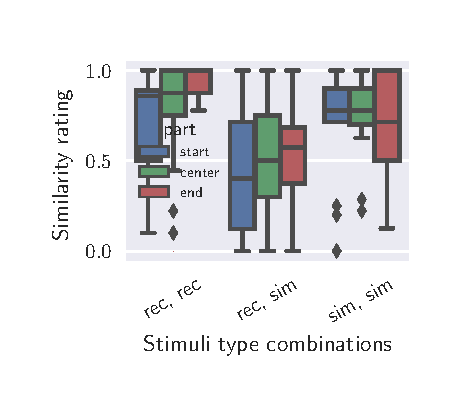
\includegraphics[]{../figures/generated/listening-analysis/figure5_ratings_part_A320}
  \caption{Similarity ratings for the A320 grouped by stimuli type combinations and stimuli part.}
  \label{fig:listening:results:ratings-A320-parts}
% \end{figure}
% TODO discuss

% \begin{figure}[H]
  \centering
  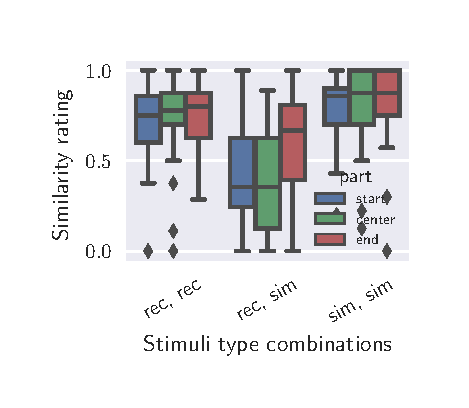
\includegraphics[]{../figures/generated/listening-analysis/figure6_ratings_part_RJ1H}
  \caption{Similarity ratings for the RJ1H grouped by stimuli type combinations and stimuli part.}
  \label{fig:listening:results:ratings-RJ1H-parts}
\end{figure}
% \end{float}
% TODO discuss
% }

\newpage
\section{Discussion}
To test whether the hypothesis is true, the distributions of similarity ratings of a

As can be seen in Figure
\ref{fig:listening:ratings-aircraft-type-combinations:recordings}, the A320's
are judged to be very similar to each other, and the RJ1H's as quite similar to
each other as well. The A320's are not rated as very similar to the RJ1H's and therefore
it appears that the participants can discriminate between the two aircraft
types.

In the case of the auralisations, Figure
\ref{fig:listening:ratings-aircraft-type-combinations:auralisations}, the
participants can also discriminate between the aircraft types, but now the
RJ1H's are judged to be relatively more similar than the A320's. Compared to the
recordings the difference between the A320's and the RJ1H's is slightly smaller.

% One might argue from these findings that the whole set of auralisations is more similar than the set of recordings.

Figures \ref{fig:listening:ratings-stimuli-type-combinations:A320} and
\ref{fig:listening:ratings-stimuli-type-combinations:RJ1H} show as additional
information how similar the auralisations are to the recordings. The groups
``(rec, sim)'' contain pairs consisting of a recording and an auralisation. The
similarity ratings for these two groups are similar to the ``(A320, RJ1H)''
groups in Figures
\ref{fig:listening:ratings-aircraft-type-combinations:recordings} and
\ref{fig:listening:ratings-aircraft-type-combinations:auralisations}. Therefore,
it would appear that listeners can discriminate between aircraft types, but that
the auralisations are considered to be of different aircraft types than the
recordings they are based on.

Figures \ref{fig:listening:results:ratings-A320-parts} and
\ref{fig:listening:results:ratings-RJ1H-parts} show the same data
but now further grouped by stimuli part. Judging from Figure
\ref{fig:listening:ratings-stimuli-type-combinations:A320} there appears to be a
relative large dissimilarity between the approach parts of the A320 recordings
and also between the ``end'' parts of the A320 auralisations. The groups ``(rec,
rec)'' and ``(sim, sim)'' consist however of only 17 data points each whereas
the ``(rec, sim)'' group has 68 data points.

The participants mentioned relatively larger differences in the stimuli that
correspond to the approach of the aircraft (``start`` stimuli). During the
approach the tonal components are clearly audible compared to other parts of the
events due to the directivity. The feature-extraction algorithm was known to
underestimate the power and bandwidth of the blade passing frequency and its
harmonics because the algorithm was tuned for the Buzz-Saw tones. Therefore, a
likely explanation is that this underestimation of power and bandwidth is
causing audible differences between recordings and auralisations.
